
\documentclass[letterpaper,hide notes,xcolor={table,svgnames},pdftex,10pt]{beamer}
\def\showexamples{t}

\usecolortheme{crane}
\setbeamertemplate{navigation symbols}{}

\usetheme{MyPittsburgh}
\usepackage{hyperref}
\usepackage{graphicx,xspace}
\usepackage[normalem]{ulem}
\usepackage{multicol}
\usepackage{amsmath,amssymb,amsthm,graphicx,xspace}
\newcommand\SF[1]{$\bigstar$\footnote{SF: #1}}

\usepackage[sfdefault,lf]{carlito}
\usepackage[T1]{fontenc}
\usepackage[scaled]{beramono}
\usepackage{tikzpagenodes}
\newcommand{\Rplus}{\protect\hspace{-.1em}\protect\raisebox{.35ex}{\small{\small\textbf{+}}}}
\newcommand{\Cpp}{\mbox{C\Rplus\Rplus}\xspace}

\newcounter{tmpnumSlide}
\newcounter{tmpnumNote}

\newcommand\mnote[1]{%
	\addtocounter{tmpnumSlide}{1}
	\ifdefined\showcues {~\tiny\fbox{\arabic{tmpnumSlide}}}\fi
	\note{\setlength{\parskip}{1ex}\addtocounter{tmpnumNote}{1}\textbf{\Large \arabic{tmpnumNote}:} {#1\par}}}

\newcommand\mmnote[1]{\note{\setlength{\parskip}{1ex}#1\par}}


\newcommand\mquestion[2]{{~\color{red}\fbox{?}}\note{\setlength{\parskip}{1ex}\par{\Large \textbf{?}} #1} \note{\setlength{\parskip}{1ex}\par{\Large \textbf{A}} #2\par}\ifdefined \presentationonly \pause \fi}

\newcommand\blackboard[1]{%
	\ifdefined   \showblackboard
		{#1}
	\else {\begin{center} \fbox{\colorbox{blue!30}{%
						\begin{minipage}{.95\linewidth}%
							\hspace{\stretch{1}} Some space intentionally left blank; done at the blackboard.%
						\end{minipage}}}\end{center}}%
	\fi%
}

\usepackage{listings}
\lstset{%
	keywordstyle=\bfseries,
	aboveskip=15pt,
	belowskip=15pt,
	captionpos=b,
	identifierstyle=\ttfamily,
	frame=lines,
	numbers=left, basicstyle=\scriptsize, numberstyle=\tiny, stepnumber=0, numbersep=2pt}

\usepackage{siunitx}
\newcommand\sius[1]{\num[group-separator = {,}]{#1}\si{\micro\second}}
\newcommand\sims[1]{\num[group-separator = {,}]{#1}\si{\milli\second}}
\newcommand\sins[1]{\num[group-separator = {,}]{#1}\si{\nano\second}}
\sisetup{group-separator = {,}, group-digits = true}

%% -------------------- tikz --------------------
\usepackage{tikz}
\usetikzlibrary{positioning}
\usetikzlibrary{arrows,backgrounds,automata,decorations.shapes,decorations.pathmorphing,decorations.markings,decorations.text}

\tikzstyle{place}=[circle,draw=blue!50,fill=blue!20,thick, inner sep=0pt,minimum size=6mm]
\tikzstyle{transition}=[rectangle,draw=black!50,fill=black!20,thick, inner sep=0pt,minimum size=4mm]

\tikzstyle{block}=[rectangle,draw=black, thick, inner sep=5pt]
\tikzstyle{bullet}=[circle,draw=black, fill=black, thin, inner sep=2pt]

\tikzstyle{pre}=[<-,shorten <=1pt,>=stealth',semithick]
\tikzstyle{post}=[->,shorten >=1pt,>=stealth',semithick]
\tikzstyle{bi}=[<->,shorten >=1pt,shorten <=1pt, >=stealth',semithick]

\tikzstyle{mut}=[-,>=stealth',semithick]

\tikzstyle{treereset}=[dashed,->, shorten >=1pt,>=stealth',thin]

\usepackage{ifmtarg}
\usepackage{xifthen}
\makeatletter
% new counter to now which frame it is within the sequence
\newcounter{multiframecounter}
% initialize buffer for previously used frame title
\gdef\lastframetitle{\textit{undefined}}
% new environment for a multi-frame
\newenvironment{multiframe}[1][]{%
	\ifthenelse{\isempty{#1}}{%
		% if no frame title was set via optional parameter,
		% only increase sequence counter by 1
		\addtocounter{multiframecounter}{1}%
	}{%
		% new frame title has been provided, thus
		% reset sequence counter to 1 and buffer frame title for later use
		\setcounter{multiframecounter}{1}%
		\gdef\lastframetitle{#1}%
	}%
	% start conventional frame environment and
	% automatically set frame title followed by sequence counter
	\begin{frame}%
		\frametitle{\lastframetitle~{\normalfont(\arabic{multiframecounter})}}%
		}{%
	\end{frame}%
}
\makeatother

\makeatletter
\newdimen\tu@tmpa%
\newdimen\ydiffl%
\newdimen\xdiffl%
\newcommand\ydiff[2]{%
	\coordinate (tmpnamea) at (#1);%
	\coordinate (tmpnameb) at (#2);%
	\pgfextracty{\tu@tmpa}{\pgfpointanchor{tmpnamea}{center}}%
	\pgfextracty{\ydiffl}{\pgfpointanchor{tmpnameb}{center}}%
	\advance\ydiffl by -\tu@tmpa%
}
\newcommand\xdiff[2]{%
	\coordinate (tmpnamea) at (#1);%
	\coordinate (tmpnameb) at (#2);%
	\pgfextractx{\tu@tmpa}{\pgfpointanchor{tmpnamea}{center}}%
	\pgfextractx{\xdiffl}{\pgfpointanchor{tmpnameb}{center}}%
	\advance\xdiffl by -\tu@tmpa%
}
\makeatother
\newcommand{\copyrightbox}[3][r]{%
	\begin{tikzpicture}%
		\node[inner sep=0pt,minimum size=2em](ciimage){#2};
		\usefont{OT1}{phv}{n}{n}\fontsize{4}{4}\selectfont
		\ydiff{ciimage.south}{ciimage.north}
		\xdiff{ciimage.west}{ciimage.east}
		\ifthenelse{\equal{#1}{r}}{%
			\node[inner sep=0pt,right=1ex of ciimage.south east,anchor=north west,rotate=90]%
			{\raggedleft\color{black!50}\parbox{\the\ydiffl}{\raggedright{}#3}};%
		}{%
			\ifthenelse{\equal{#1}{l}}{%
				\node[inner sep=0pt,right=1ex of ciimage.south west,anchor=south west,rotate=90]%
				{\raggedleft\color{black!50}\parbox{\the\ydiffl}{\raggedright{}#3}};%
			}{%
				\node[inner sep=0pt,below=1ex of ciimage.south west,anchor=north west]%
				{\raggedleft\color{black!50}\parbox{\the\xdiffl}{\raggedright{}#3}};%
			}
		}
	\end{tikzpicture}
}


%% --------------------

%\usepackage[excludeor]{everyhook}
%\PushPreHook{par}{\setbox0=\lastbox\llap{MUH}}\box0}

%\vspace*{\stretch{1}

%\setbox0=\lastbox \llap{\textbullet\enskip}\box0}

\setlength{\parskip}{\fill}

\newcommand\noskips{\setlength{\parskip}{1ex}}
\newcommand\doskips{\setlength{\parskip}{\fill}}

\newcommand\xx{\par\vspace*{\stretch{1}}\par}
\newcommand\xxs{\par\vspace*{2ex}\par}
\newcommand\tuple[1]{\langle #1 \rangle}
\newcommand\code[1]{{\sf \footnotesize #1}}
\newcommand\ex[1]{\uline{Example:} \ifdefined \presentationonly \pause \fi
	\ifdefined\showexamples#1\xspace\else{\uline{\hspace*{2cm}}}\fi}

\newcommand\ceil[1]{\lceil #1 \rceil}


\AtBeginSection[]
{
	\begin{frame}
		\frametitle{Outline}
		\tableofcontents[currentsection]
	\end{frame}
}



\pgfdeclarelayer{edgelayer}
\pgfdeclarelayer{nodelayer}
\pgfsetlayers{edgelayer,nodelayer,main}

\tikzstyle{none}=[inner sep=0pt]
\tikzstyle{rn}=[circle,fill=Red,draw=Black,line width=0.8 pt]
\tikzstyle{gn}=[circle,fill=Lime,draw=Black,line width=0.8 pt]
\tikzstyle{yn}=[circle,fill=Yellow,draw=Black,line width=0.8 pt]
\tikzstyle{empty}=[circle,fill=White,draw=Black]
\tikzstyle{bw} = [rectangle, draw, fill=blue!20,
text width=4em, text centered, rounded corners, minimum height=2em]

\newcommand{\CcNote}[1]{% longname
	This work is licensed under the \textit{Creative Commons #1 3.0 License}.%
}
\newcommand{\CcImageBy}[1]{%
	\includegraphics[scale=#1]{creative_commons/cc_by_30.pdf}%
}
\newcommand{\CcImageSa}[1]{%
	\includegraphics[scale=#1]{creative_commons/cc_sa_30.pdf}%
}
\newcommand{\CcImageNc}[1]{%
	\includegraphics[scale=#1]{creative_commons/cc_nc_30.pdf}%
}
\newcommand{\CcGroupBySa}[2]{% zoom, gap
	\CcImageBy{#1}\hspace*{#2}\CcImageNc{#1}\hspace*{#2}\CcImageSa{#1}%
}
\newcommand{\CcLongnameByNcSa}{Attribution-NonCommercial-ShareAlike}

\newenvironment{changemargin}[1]{% 
	\begin{list}{}{% 
		\setlength{\topsep}{0pt}% 
		\setlength{\leftmargin}{#1}% 
		\setlength{\rightmargin}{1em}
		\setlength{\listparindent}{\parindent}% 
		\setlength{\itemindent}{\parindent}% 
		      \setlength{\parsep}{\parskip}% 
		      }% 
		\item[]}{\end{list}}




\title{Lecture 32 --- Event-Driven I/O with libevent }

\author{Jeff Zarnett \\ \small \texttt{jzarnett@uwaterloo.ca}}
\institute{Department of Electrical and Computer Engineering \\
  University of Waterloo}
\date{\today}


\begin{document}

\begin{frame}
  \titlepage

 \end{frame}



\begin{frame}
\frametitle{Events!}

\begin{center}
	
\includegraphics[width=0.5\textwidth]{images/invitation}
\end{center}


\end{frame}


\begin{frame}
\frametitle{Using libevent}

The libevent library is meant for high performance applications and scalable network servers. 

Instead of focusing now on whether an operation is blocking or not, we'll try to think about I/O as events: when something happens, take some action.

\end{frame}


\begin{frame}[fragile]
\frametitle{Let's Get Ready}
The library supports a lot of different configuration options.

But the most important setup thing is that we need to configure it to use the pthreads library and functions.

\begin{lstlisting}[language=C]
int evthread_use_pthreads( )
\end{lstlisting}

\end{frame}


\begin{frame}
\frametitle{Zero Wing...}

\begin{center}
	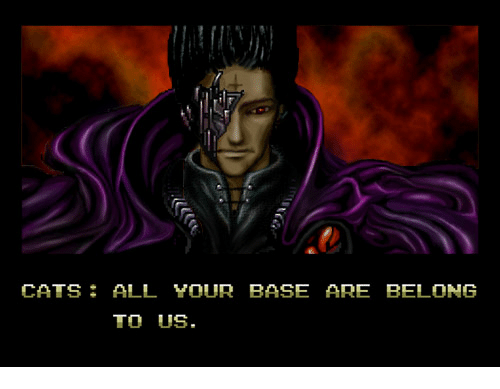
\includegraphics[width=0.6\textwidth]{images/allyourbase.png}
\end{center}

Each event is associated with an \texttt{event\_base} structure.

We might need multiple bases for multiple thread operations.

\end{frame}

\begin{frame}[fragile]
\frametitle{Building a Base}

\begin{lstlisting}[language=C]
struct event_base* event_base_new( ); /* Create with default settings */
struct event_base* event_base_new_with_config( 
    const struct event_config* cfg ); /* Create with configuration */
struct event_config* event_config_new( );
void event_config_free( struct event_config* cfg );
\end{lstlisting} 

The use of a configuration is optional.

To deallocate an event base, the (self-explanatory) function for that is:
\begin{lstlisting}[language=C]
void event_base_free( struct event_base* base );
\end{lstlisting}

\end{frame}


\begin{frame}[fragile]
\frametitle{Find Your Team's Capabilities}
\begin{lstlisting}[language=C]
#include <stdlib.h>
#include <stdio.h>
#include <event2/event.h>

int main( int argc, char** argv ) { 

    int i;
    const char **methods = event_get_supported_methods();
    printf("Starting Libevent %s.  Available methods are:\n",
            event_get_version());
    for (i=0; methods[i] != NULL; ++i) {
        printf("    %s\n", methods[i]);
    }   
    return 0;
}
\end{lstlisting}

\end{frame}

\begin{frame}[fragile]
\frametitle{Ask \texttt{ecetesla0}}

{\small
\begin{verbatim}
jzarnett@ecetesla0:~/ece252$ gcc -std=c99 -g -levent -o le1 le1.c
jzarnett@ecetesla0:~/ece252$ ./le1 
Starting Libevent 2.1.8-stable.  Available methods are:
    epoll
    poll
    select
\end{verbatim}
}

\end{frame}

\begin{frame}[fragile]
\frametitle{What You Can Do vs What You Will Do}

\begin{lstlisting}[language=C]
#include <stdlib.h>
#include <stdio.h>
#include <event2/event.h>

int main( int argc, char** argv ) { 
    struct event_base *base;
    enum event_method_feature f;

    base = event_base_new();
    if (!base) {
        puts("Couldn't get an event_base!");
    } else {
        printf("Using Libevent with backend method %s.",
                event_base_get_method(base));
        f = event_base_get_features(base);
        if ((f & EV_FEATURE_ET))
            printf("  Edge-triggered events are supported.");
        if ((f & EV_FEATURE_O1))
            printf("  O(1) event notification is supported.");
        if ((f & EV_FEATURE_FDS))
            printf("  All FD types are supported.");
        puts("");
    }   
    return 0;
}
\end{lstlisting}


\end{frame}

\begin{frame}[fragile]
\frametitle{Well, we'll... just go with that then.}

\begin{verbatim}
jzarnett@ecetesla0:~/ece252$ ./le2
Using Libevent with backend method epoll.  
 Edge-triggered events are supported.  
 O(1) event notification is supported.
\end{verbatim}

Wait, we didn't learn about epoll... Do we need to?

\end{frame}


\begin{frame}
\frametitle{Cancel Red Alert}

No.

The great thing about libevent is that we don't have to think about the details of the backend.


\end{frame}


\begin{frame}
\frametitle{Keep Your Eyes Open}

The goal is to watch for some events; for that we need a definition of an event. 

An event happens on a file descriptor (as usual). 

Event Lifecycle:\begin{itemize}
	\item Created
	\item Initialized
	\item Pending
	\item Non-Pending
\end{itemize}

\end{frame}


\begin{frame}[fragile]
\frametitle{Creating an Event Events}

\begin{lstlisting}[language=C]
typedef void (*event_callback_fn)( evutil_socket_t fd, short what, void* arg )
struct event* event_new( struct event_base* base, evutil_socket_t fd, 
    short what, event_callback_fn cb, void* arg )
\end{lstlisting}


\texttt{event\_callback\_fn}: function signature definition for callback.

\texttt{base}: event base to use.

\texttt{fd}: file descriptor.

\texttt{what}: what we want to be notified of.

\texttt{arg}: user-defined argument.

\end{frame}


\begin{frame}
\frametitle{What?!}

\begin{center}
	
\includegraphics[width=0.7\textwidth]{images/short.jpg}
\end{center}

\end{frame}


\begin{frame}[fragile]
\frametitle{The what Parameter}

\begin{lstlisting}[language=C]
#define EV_TIMEOUT      0x01
#define EV_READ         0x02
#define EV_WRITE        0x04
#define EV_SIGNAL       0x08
#define EV_PERSIST      0x10
#define EV_ET           0x20
\end{lstlisting}

Some require some explanation...


They can be combined with the bitwise-OR operator again.

\end{frame}


\begin{frame}
\frametitle{Call Yourself?}

If you want the event itself to be the \texttt{void*} argument passed to the callback function, that can be done here as well. 

Normally this would not work, because the event doesn't exist yet. 

But there's a workaround for that, a function \texttt{event\_self\_cbarg()} that does a little magic for you.

\end{frame}


\begin{frame}[fragile]
\frametitle{Destroying an Event}
\begin{lstlisting}[language=C]
void event_free( struct event* event )
\end{lstlisting}

It is okay to call this even on an event that is pending or active.

\end{frame}


\begin{frame}[fragile]
\frametitle{Ready to Watch? Done Watching?}

\begin{lstlisting}[language=C]
int event_add( struct event* ev, const struct timeval* tv );
int event_del( struct event* ev );
\end{lstlisting}

But did we forget something?

Oh yeah... starting the events!

\end{frame}


\begin{frame}[fragile]
\frametitle{Dispatching Events}

There are two ways to dispatch events, the simple way and the hard way:
\begin{lstlisting}[language=C]
int event_base_dispatch( struct event_base* base);
int event_base_loop(struct event_base *base, int flags);
\end{lstlisting}

The easy way is the same as the hard way with no flags set.

\begin{lstlisting}[language=C]
#define EVLOOP_ONCE             0x01
#define EVLOOP_NONBLOCK         0x02
#define EVLOOP_NO_EXIT_ON_EMPTY 0x04
\end{lstlisting}

No-exit means don't break the loop when no more events pending/active.

\end{frame}


\begin{frame}[fragile]
\frametitle{When I Say...}

\begin{center}
	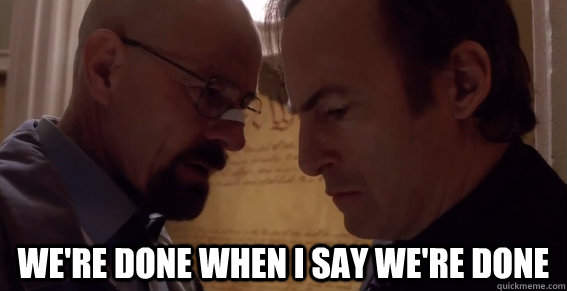
\includegraphics[width=0.4\textwidth]{images/whenisay.jpg}
\end{center}

\begin{lstlisting}[language=C]
int event_base_loopexit(struct event_base* base, const struct timeval* tv);
int event_base_loopbreak(struct event_base* base);
\end{lstlisting}


\end{frame}


\begin{frame}[fragile]
\frametitle{Start Events and Watch For Them}

\begin{lstlisting}[language=C]
void cb_func( evutil_socket_t fd, short what, void *arg ) {
        const char *data = arg;
        printf("Got an event on socket %d:%s%s%s%s [%s]",
            (int) fd,
            (what&EV_TIMEOUT) ? " timeout" : "",
            (what&EV_READ)    ? " read" : "",
            (what&EV_WRITE)   ? " write" : "",
            (what&EV_SIGNAL)  ? " signal" : "",
            data);
}
\end{lstlisting}
\end{frame}

\begin{frame}[fragile]
\frametitle{Start Events and Watch For Them}
\begin{lstlisting}[language=C]
void main_loop( evutil_socket_t fd1, evutil_socket_t fd2 ){
        struct event *ev1, *ev2;
        struct timeval five_seconds = {5,0};
        struct event_base *base = event_base_new();

        /* The caller has already set up fd1, fd2 somehow, 
           and make them nonblocking. */

        ev1 = event_new(base, fd1, EV_TIMEOUT|EV_READ|EV_PERSIST, cb_func,
            (char*)"Reading event");
        ev2 = event_new(base, fd2, EV_WRITE|EV_PERSIST, cb_func, 
            (char*)"Writing event");

        event_add(ev1, &five_seconds);
        event_add(ev2, NULL);
        event_base_dispatch(base);
}
\end{lstlisting} 

\end{frame}


\begin{frame}[fragile]
\frametitle{It's Clean-Up Time}

Finally, libevent has some global structures that are initialized once. 

When we're all completely done with everything:

\begin{lstlisting}[language=C]
void libevent_global_shutdown( )
\end{lstlisting}

This does not deallocate anything that was the return value of a libevent function.

\end{frame}



\begin{frame}
\frametitle{Buffering...}

\begin{center}
	
\includegraphics[width=0.5\textwidth]{images/buffering.jpeg}
\end{center}


We might want to wait until we have a significant chunk of data before we're ready to process it.

\end{frame}


\begin{frame}
\frametitle{Buffering...}

It's better to have the event happen when a condition is fulfilled, such as having enough data available.

The library does support this: \texttt{bufferevents}!

A normal callback is triggered when the underlying transport (e.g., socket) is ready to be read or written.

A buffer event takes place when enough data has been read or written.

Buffer events really only work for TCP communication.

\end{frame}


\begin{frame}
\frametitle{Always Two, There Are}

Each buffer event has two buffers: the input and output buffer.

There are also two callbacks, a read and a write callback.

There are defaults; these can be overridden.

\end{frame}


\begin{frame}
\frametitle{Watermarks}

Every buffer event has four ``watermarks'':
\begin{itemize}
	\item Read low-water mark
	\item Read high-water mark
	\item Write low-water mark
	\item Write high-water mark
\end{itemize}


\end{frame}


\begin{frame}[fragile]
\frametitle{Make Me a Buffer Event}

\begin{lstlisting}[language=C]
struct bufferevent* bufferevent_socket_new( struct event_base* base, 
    evutil_socket_t fd, enum bufferevent_options options );
\end{lstlisting}

\texttt{base}: the event base the buffer event belongs too.

\texttt{fd}: file descriptor

\texttt{options}: there are several, but we care about \texttt{BEV\_OPT\_CLOSE\_ON\_FREE}, \texttt{BEV\_OPT\_THREADSAFE}


\begin{lstlisting}[language=C]
void bufferevent_free( struct bufferevent* bev );
\end{lstlisting}

Deallocation is straightforward...
\end{frame}

\begin{frame}[fragile]
\frametitle{Callbacks}

\begin{lstlisting}[language=C]
typedef void (*bufferevent_data_cb)(struct bufferevent* bev, void* ctx);
typedef void (*bufferevent_event_cb)(struct bufferevent* bev, 
     short events, void* ctx);
\end{lstlisting}

Return type is void.

\texttt{bev}: buffer event in question.

\texttt{ctx}: user-provided context.

\texttt{what}: same as before, what we are interested in,.

\end{frame}


\begin{frame}[fragile]
\frametitle{Set up Buffer Event Callbacks}

\begin{lstlisting}[language=C]
void bufferevent_setcb(struct bufferevent* bufev, 
    bufferevent_data_cb readcb, bufferevent_data_cb writecb, 
    bufferevent_event_cb eventcb, void* cbarg);
\end{lstlisting}

\texttt{bufev}: buffer event in question

\texttt{readcb}: read callback, \texttt{NULL} if not desired.

\texttt{writecb}: write callback; \texttt{NULL} if not desired.

\texttt{eventcb}: event callback; \texttt{NULL} if not desired.

\texttt{cbarg}: the user-supplied argument.

\end{frame}


\begin{frame}[fragile]
\frametitle{Now We're Ready...}

We're ready, but have not yet actually created the event.

\begin{lstlisting}[language=C]
int bufferevent_socket_connect( struct bufferevent* bev, 
    struct sockaddr* address, int addrlen );
\end{lstlisting}

\texttt{bev}: buffer event in question.

\texttt{address}: address to connect to.

\texttt{addrlen}: size of the address structure.

\end{frame}


\begin{frame}[fragile]
\frametitle{Put It All Together: A Silly Callback}


\begin{lstlisting}[language=C]
#include <event2/event.h>
#include <event2/bufferevent.h>
#include <sys/socket.h>
#include <string.h>

void eventcb(struct bufferevent *bev, short events, void *ptr) {
    if (events & BEV_EVENT_CONNECTED) {
         /* We're connected to 127.0.0.1:8080.   Ordinarily we'd do
            something here, like start reading or writing. */
    } else if (events & BEV_EVENT_ERROR) {
         /* An error occured while connecting. */
    }
}
\end{lstlisting}

\end{frame}

\begin{frame}[fragile]
\frametitle{Put It All Together: Main Loop}

\begin{lstlisting}[language=C]
int main_loop( ) {
    struct event_base *base;
    struct bufferevent *bev;
    struct sockaddr_in sin;

    base = event_base_new();

    memset(&sin, 0, sizeof(sin));
    sin.sin_family = AF_INET;
    sin.sin_addr.s_addr = htonl(0x7f000001); /* 127.0.0.1 */
    sin.sin_port = htons(8080); /* Port 8080 */

    bev = bufferevent_socket_new(base, -1, BEV_OPT_CLOSE_ON_FREE);

    bufferevent_setcb(bev, NULL, NULL, eventcb, NULL);

    if (bufferevent_socket_connect(bev,
        (struct sockaddr *)&sin, sizeof(sin)) < 0) {
        /* Error starting connection */
        bufferevent_free(bev);
        return -1;
    }

    event_base_dispatch(base);
    return 0;
}\end{lstlisting}

\end{frame}


\begin{frame}
\frametitle{This Is Just The Beginning}

By no means have we covered every possible option or tool in the libevent library.

It's just one of the many ways we have seen for how to do asynchronous I/O...


\end{frame}


\begin{frame}
\frametitle{Sunset in Starling City...}

\begin{center}
	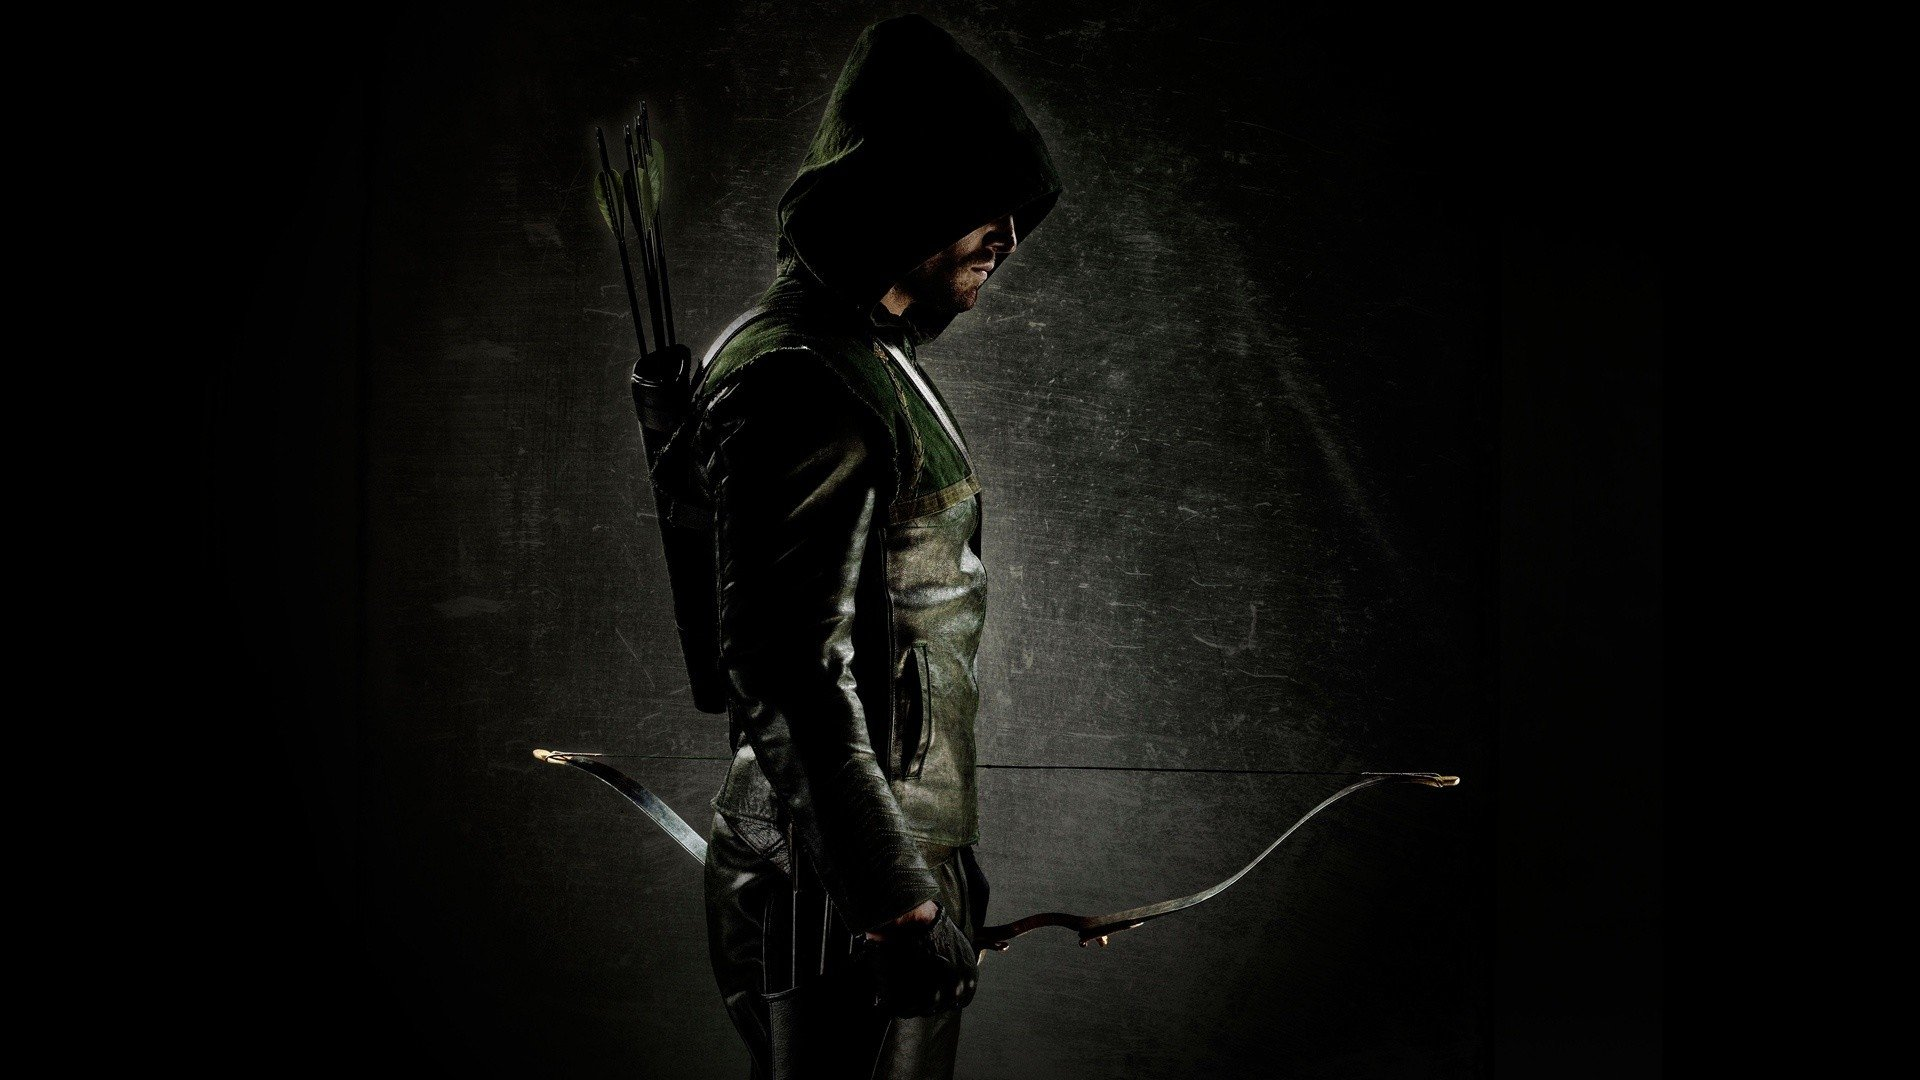
\includegraphics[width=\textwidth]{images/arrow.jpg}
\end{center}

\end{frame}


\end{document}

